% Options for packages loaded elsewhere
\PassOptionsToPackage{unicode}{hyperref}
\PassOptionsToPackage{hyphens}{url}
\PassOptionsToPackage{dvipsnames,svgnames,x11names}{xcolor}
%
\documentclass[
  letterpaper,
  DIV=11,
  numbers=noendperiod]{scrartcl}

\usepackage{amsmath,amssymb}
\usepackage{lmodern}
\usepackage{iftex}
\ifPDFTeX
  \usepackage[T1]{fontenc}
  \usepackage[utf8]{inputenc}
  \usepackage{textcomp} % provide euro and other symbols
\else % if luatex or xetex
  \usepackage{unicode-math}
  \defaultfontfeatures{Scale=MatchLowercase}
  \defaultfontfeatures[\rmfamily]{Ligatures=TeX,Scale=1}
\fi
% Use upquote if available, for straight quotes in verbatim environments
\IfFileExists{upquote.sty}{\usepackage{upquote}}{}
\IfFileExists{microtype.sty}{% use microtype if available
  \usepackage[]{microtype}
  \UseMicrotypeSet[protrusion]{basicmath} % disable protrusion for tt fonts
}{}
\makeatletter
\@ifundefined{KOMAClassName}{% if non-KOMA class
  \IfFileExists{parskip.sty}{%
    \usepackage{parskip}
  }{% else
    \setlength{\parindent}{0pt}
    \setlength{\parskip}{6pt plus 2pt minus 1pt}}
}{% if KOMA class
  \KOMAoptions{parskip=half}}
\makeatother
\usepackage{xcolor}
\setlength{\emergencystretch}{3em} % prevent overfull lines
\setcounter{secnumdepth}{-\maxdimen} % remove section numbering
% Make \paragraph and \subparagraph free-standing
\ifx\paragraph\undefined\else
  \let\oldparagraph\paragraph
  \renewcommand{\paragraph}[1]{\oldparagraph{#1}\mbox{}}
\fi
\ifx\subparagraph\undefined\else
  \let\oldsubparagraph\subparagraph
  \renewcommand{\subparagraph}[1]{\oldsubparagraph{#1}\mbox{}}
\fi

\usepackage{color}
\usepackage{fancyvrb}
\newcommand{\VerbBar}{|}
\newcommand{\VERB}{\Verb[commandchars=\\\{\}]}
\DefineVerbatimEnvironment{Highlighting}{Verbatim}{commandchars=\\\{\}}
% Add ',fontsize=\small' for more characters per line
\usepackage{framed}
\definecolor{shadecolor}{RGB}{241,243,245}
\newenvironment{Shaded}{\begin{snugshade}}{\end{snugshade}}
\newcommand{\AlertTok}[1]{\textcolor[rgb]{0.68,0.00,0.00}{#1}}
\newcommand{\AnnotationTok}[1]{\textcolor[rgb]{0.37,0.37,0.37}{#1}}
\newcommand{\AttributeTok}[1]{\textcolor[rgb]{0.40,0.45,0.13}{#1}}
\newcommand{\BaseNTok}[1]{\textcolor[rgb]{0.68,0.00,0.00}{#1}}
\newcommand{\BuiltInTok}[1]{\textcolor[rgb]{0.00,0.23,0.31}{#1}}
\newcommand{\CharTok}[1]{\textcolor[rgb]{0.13,0.47,0.30}{#1}}
\newcommand{\CommentTok}[1]{\textcolor[rgb]{0.37,0.37,0.37}{#1}}
\newcommand{\CommentVarTok}[1]{\textcolor[rgb]{0.37,0.37,0.37}{\textit{#1}}}
\newcommand{\ConstantTok}[1]{\textcolor[rgb]{0.56,0.35,0.01}{#1}}
\newcommand{\ControlFlowTok}[1]{\textcolor[rgb]{0.00,0.23,0.31}{#1}}
\newcommand{\DataTypeTok}[1]{\textcolor[rgb]{0.68,0.00,0.00}{#1}}
\newcommand{\DecValTok}[1]{\textcolor[rgb]{0.68,0.00,0.00}{#1}}
\newcommand{\DocumentationTok}[1]{\textcolor[rgb]{0.37,0.37,0.37}{\textit{#1}}}
\newcommand{\ErrorTok}[1]{\textcolor[rgb]{0.68,0.00,0.00}{#1}}
\newcommand{\ExtensionTok}[1]{\textcolor[rgb]{0.00,0.23,0.31}{#1}}
\newcommand{\FloatTok}[1]{\textcolor[rgb]{0.68,0.00,0.00}{#1}}
\newcommand{\FunctionTok}[1]{\textcolor[rgb]{0.28,0.35,0.67}{#1}}
\newcommand{\ImportTok}[1]{\textcolor[rgb]{0.00,0.46,0.62}{#1}}
\newcommand{\InformationTok}[1]{\textcolor[rgb]{0.37,0.37,0.37}{#1}}
\newcommand{\KeywordTok}[1]{\textcolor[rgb]{0.00,0.23,0.31}{#1}}
\newcommand{\NormalTok}[1]{\textcolor[rgb]{0.00,0.23,0.31}{#1}}
\newcommand{\OperatorTok}[1]{\textcolor[rgb]{0.37,0.37,0.37}{#1}}
\newcommand{\OtherTok}[1]{\textcolor[rgb]{0.00,0.23,0.31}{#1}}
\newcommand{\PreprocessorTok}[1]{\textcolor[rgb]{0.68,0.00,0.00}{#1}}
\newcommand{\RegionMarkerTok}[1]{\textcolor[rgb]{0.00,0.23,0.31}{#1}}
\newcommand{\SpecialCharTok}[1]{\textcolor[rgb]{0.37,0.37,0.37}{#1}}
\newcommand{\SpecialStringTok}[1]{\textcolor[rgb]{0.13,0.47,0.30}{#1}}
\newcommand{\StringTok}[1]{\textcolor[rgb]{0.13,0.47,0.30}{#1}}
\newcommand{\VariableTok}[1]{\textcolor[rgb]{0.07,0.07,0.07}{#1}}
\newcommand{\VerbatimStringTok}[1]{\textcolor[rgb]{0.13,0.47,0.30}{#1}}
\newcommand{\WarningTok}[1]{\textcolor[rgb]{0.37,0.37,0.37}{\textit{#1}}}

\providecommand{\tightlist}{%
  \setlength{\itemsep}{0pt}\setlength{\parskip}{0pt}}\usepackage{longtable,booktabs,array}
\usepackage{calc} % for calculating minipage widths
% Correct order of tables after \paragraph or \subparagraph
\usepackage{etoolbox}
\makeatletter
\patchcmd\longtable{\par}{\if@noskipsec\mbox{}\fi\par}{}{}
\makeatother
% Allow footnotes in longtable head/foot
\IfFileExists{footnotehyper.sty}{\usepackage{footnotehyper}}{\usepackage{footnote}}
\makesavenoteenv{longtable}
\usepackage{graphicx}
\makeatletter
\def\maxwidth{\ifdim\Gin@nat@width>\linewidth\linewidth\else\Gin@nat@width\fi}
\def\maxheight{\ifdim\Gin@nat@height>\textheight\textheight\else\Gin@nat@height\fi}
\makeatother
% Scale images if necessary, so that they will not overflow the page
% margins by default, and it is still possible to overwrite the defaults
% using explicit options in \includegraphics[width, height, ...]{}
\setkeys{Gin}{width=\maxwidth,height=\maxheight,keepaspectratio}
% Set default figure placement to htbp
\makeatletter
\def\fps@figure{htbp}
\makeatother

\KOMAoption{captions}{tableheading}
\makeatletter
\makeatother
\makeatletter
\makeatother
\makeatletter
\@ifpackageloaded{caption}{}{\usepackage{caption}}
\AtBeginDocument{%
\ifdefined\contentsname
  \renewcommand*\contentsname{Table of contents}
\else
  \newcommand\contentsname{Table of contents}
\fi
\ifdefined\listfigurename
  \renewcommand*\listfigurename{List of Figures}
\else
  \newcommand\listfigurename{List of Figures}
\fi
\ifdefined\listtablename
  \renewcommand*\listtablename{List of Tables}
\else
  \newcommand\listtablename{List of Tables}
\fi
\ifdefined\figurename
  \renewcommand*\figurename{Figure}
\else
  \newcommand\figurename{Figure}
\fi
\ifdefined\tablename
  \renewcommand*\tablename{Table}
\else
  \newcommand\tablename{Table}
\fi
}
\@ifpackageloaded{float}{}{\usepackage{float}}
\floatstyle{ruled}
\@ifundefined{c@chapter}{\newfloat{codelisting}{h}{lop}}{\newfloat{codelisting}{h}{lop}[chapter]}
\floatname{codelisting}{Listing}
\newcommand*\listoflistings{\listof{codelisting}{List of Listings}}
\makeatother
\makeatletter
\@ifpackageloaded{caption}{}{\usepackage{caption}}
\@ifpackageloaded{subcaption}{}{\usepackage{subcaption}}
\makeatother
\makeatletter
\@ifpackageloaded{tcolorbox}{}{\usepackage[many]{tcolorbox}}
\makeatother
\makeatletter
\@ifundefined{shadecolor}{\definecolor{shadecolor}{rgb}{.97, .97, .97}}
\makeatother
\makeatletter
\makeatother
\ifLuaTeX
  \usepackage{selnolig}  % disable illegal ligatures
\fi
\IfFileExists{bookmark.sty}{\usepackage{bookmark}}{\usepackage{hyperref}}
\IfFileExists{xurl.sty}{\usepackage{xurl}}{} % add URL line breaks if available
\urlstyle{same} % disable monospaced font for URLs
\hypersetup{
  pdftitle={Class09 Structural Bioinformatics},
  pdfauthor={Mady Welch},
  colorlinks=true,
  linkcolor={blue},
  filecolor={Maroon},
  citecolor={Blue},
  urlcolor={Blue},
  pdfcreator={LaTeX via pandoc}}

\title{Class09 Structural Bioinformatics}
\author{Mady Welch}
\date{}

\begin{document}
\maketitle
\ifdefined\Shaded\renewenvironment{Shaded}{\begin{tcolorbox}[boxrule=0pt, frame hidden, sharp corners, enhanced, interior hidden, borderline west={3pt}{0pt}{shadecolor}, breakable]}{\end{tcolorbox}}\fi

\hypertarget{pdb-statistics}{%
\subsection{PDB Statistics}\label{pdb-statistics}}

Download a CSV file from the PDB site and open it:

\begin{Shaded}
\begin{Highlighting}[]
\NormalTok{PdbStats }\OtherTok{\textless{}{-}} \FunctionTok{read.csv}\NormalTok{(}\StringTok{"Data Export Summary.csv"}\NormalTok{)}
\NormalTok{PdbStats}
\end{Highlighting}
\end{Shaded}

\begin{verbatim}
           Molecular.Type   X.ray    NMR    EM Multiple.methods Neutron Other
1          Protein (only) 150,342 12,053 8,534              188      72    32
2 Protein/Oligosaccharide   8,866     32 1,540                6       0     0
3              Protein/NA   7,911    278 2,681                6       0     0
4     Nucleic acid (only)   2,510  1,425    74               13       2     1
5                   Other     154     31     6                0       0     0
6  Oligosaccharide (only)      11      6     0                1       0     4
    Total
1 171,221
2  10,444
3  10,876
4   4,025
5     191
6      22
\end{verbatim}

\begin{quote}
Q1. What percentage of structures in the PDB are solved by X-Ray and
Electron Microscopy?
\end{quote}

\begin{Shaded}
\begin{Highlighting}[]
\NormalTok{PdbStats}\SpecialCharTok{$}\NormalTok{X.ray}
\end{Highlighting}
\end{Shaded}

\begin{verbatim}
[1] "150,342" "8,866"   "7,911"   "2,510"   "154"     "11"     
\end{verbatim}

\begin{Shaded}
\begin{Highlighting}[]
\NormalTok{PdbStats}\SpecialCharTok{$}\NormalTok{EM}
\end{Highlighting}
\end{Shaded}

\begin{verbatim}
[1] "8,534" "1,540" "2,681" "74"    "6"     "0"    
\end{verbatim}

\begin{Shaded}
\begin{Highlighting}[]
\NormalTok{PdbStats}\SpecialCharTok{$}\NormalTok{Total}
\end{Highlighting}
\end{Shaded}

\begin{verbatim}
[1] "171,221" "10,444"  "10,876"  "4,025"   "191"     "22"     
\end{verbatim}

\begin{Shaded}
\begin{Highlighting}[]
\NormalTok{((}\DecValTok{150342} \SpecialCharTok{+} \DecValTok{8866} \SpecialCharTok{+} \DecValTok{7911} \SpecialCharTok{+} \DecValTok{2510} \SpecialCharTok{+} \DecValTok{154} \SpecialCharTok{+} \DecValTok{11} \SpecialCharTok{+} \DecValTok{8534} \SpecialCharTok{+} \DecValTok{1540} \SpecialCharTok{+} \DecValTok{2681} \SpecialCharTok{+} \DecValTok{74} \SpecialCharTok{+} \DecValTok{6} \SpecialCharTok{+} \DecValTok{0}\NormalTok{)}\SpecialCharTok{/}\NormalTok{(}\DecValTok{171221} \SpecialCharTok{+} \DecValTok{10444} \SpecialCharTok{+} \DecValTok{10876} \SpecialCharTok{+} \DecValTok{4025} \SpecialCharTok{+} \DecValTok{191} \SpecialCharTok{+} \DecValTok{22}\NormalTok{))}\SpecialCharTok{*}\DecValTok{100}
\end{Highlighting}
\end{Shaded}

\begin{verbatim}
[1] 92.80919
\end{verbatim}

\begin{itemize}
\tightlist
\item
  92.81\% of structures in the PDB are solved by X-ray and Electron
  Microscopy.
\end{itemize}

\begin{quote}
Q2. What proportion of structures in the PDB are protein?
\end{quote}

\begin{Shaded}
\begin{Highlighting}[]
\NormalTok{(}\DecValTok{171221} \SpecialCharTok{/}\NormalTok{ (}\DecValTok{171221} \SpecialCharTok{+} \DecValTok{10444} \SpecialCharTok{+} \DecValTok{10876} \SpecialCharTok{+} \DecValTok{4025} \SpecialCharTok{+} \DecValTok{191} \SpecialCharTok{+} \DecValTok{22}\NormalTok{))}\SpecialCharTok{*}\DecValTok{100}
\end{Highlighting}
\end{Shaded}

\begin{verbatim}
[1] 87.01183
\end{verbatim}

\begin{itemize}
\tightlist
\item
  87.01\% structures are protein.
\end{itemize}

\begin{quote}
Q3. Type HIV in the PDB website search box on the home page and
determine how many HIV-1 protease structures are in the current PDB?
\end{quote}

\begin{itemize}
\tightlist
\item
  4,703 structures.
\end{itemize}

\hypertarget{visualizing-the-hiv-1-protease-structure}{%
\subsection{Visualizing the HIV-1 Protease
Structure}\label{visualizing-the-hiv-1-protease-structure}}

\hypertarget{using-mol}{%
\subsubsection{Using Mol*}\label{using-mol}}

\textbf{The important role of water}

\begin{quote}
Q4. Water molecules normally have 3 atoms. Why do we see just one atom
per water molecule in this structure?
\end{quote}

\begin{itemize}
\tightlist
\item
  Because hydrogen atoms are so small, we are not able to see them in
  the structure.
\end{itemize}

\begin{quote}
Q5. There is a critical ``conserved'' water molecule in the binding
site. Can you identify this water molecule? What residue number does
this water molecule have?
\end{quote}

\begin{itemize}
\tightlist
\item
  HOH 308
\end{itemize}

Now you should be able to produce an image similar or even superior to
Figure 2 and save it to an image file.

\begin{quote}
Q6. Generate and save a figure clearly showing the two distinct chains
of HIV-protease along with the ligand. You might also consider showing
the catalytic residues ASP 25 in each chain (we recommend ``Ball \&
Stick'' for these side-chains). Add this figure to your Quarto document.
\end{quote}

\begin{figure}

{\centering 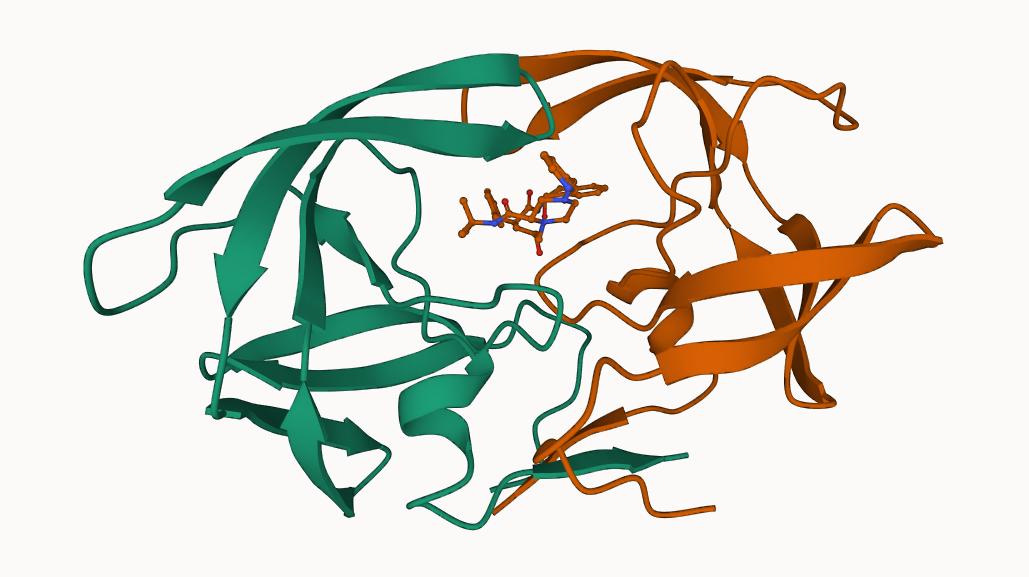
\includegraphics{1HSG.png}

}

\caption{HIV-Pr structure from 1HSG}

\end{figure}

\hypertarget{introduction-to-bio3d-in-r}{%
\subsection{Introduction to Bio3D in
R}\label{introduction-to-bio3d-in-r}}

Bio3D is an R package for structural bioinformatics. To use it we need
to call it up with \texttt{library()}

\begin{Shaded}
\begin{Highlighting}[]
\FunctionTok{library}\NormalTok{(bio3d)}
\end{Highlighting}
\end{Shaded}

To read a PDB file we can use \texttt{read.pdb()}

\begin{Shaded}
\begin{Highlighting}[]
\NormalTok{pdb }\OtherTok{\textless{}{-}} \FunctionTok{read.pdb}\NormalTok{(}\StringTok{"1hsg"}\NormalTok{)}
\end{Highlighting}
\end{Shaded}

\begin{verbatim}
  Note: Accessing on-line PDB file
\end{verbatim}

\begin{Shaded}
\begin{Highlighting}[]
\NormalTok{pdb}
\end{Highlighting}
\end{Shaded}

\begin{verbatim}

 Call:  read.pdb(file = "1hsg")

   Total Models#: 1
     Total Atoms#: 1686,  XYZs#: 5058  Chains#: 2  (values: A B)

     Protein Atoms#: 1514  (residues/Calpha atoms#: 198)
     Nucleic acid Atoms#: 0  (residues/phosphate atoms#: 0)

     Non-protein/nucleic Atoms#: 172  (residues: 128)
     Non-protein/nucleic resid values: [ HOH (127), MK1 (1) ]

   Protein sequence:
      PQITLWQRPLVTIKIGGQLKEALLDTGADDTVLEEMSLPGRWKPKMIGGIGGFIKVRQYD
      QILIEICGHKAIGTVLVGPTPVNIIGRNLLTQIGCTLNFPQITLWQRPLVTIKIGGQLKE
      ALLDTGADDTVLEEMSLPGRWKPKMIGGIGGFIKVRQYDQILIEICGHKAIGTVLVGPTP
      VNIIGRNLLTQIGCTLNF

+ attr: atom, xyz, seqres, helix, sheet,
        calpha, remark, call
\end{verbatim}

\begin{quote}
Q7: How many amino acid residues are there in this pdb object?
\end{quote}

\begin{itemize}
\tightlist
\item
  198
\end{itemize}

\begin{quote}
Q8: Name one of the two non-protein residues?
\end{quote}

\begin{itemize}
\tightlist
\item
  HOH
\end{itemize}

\begin{quote}
Q9: How many protein chains are in this structure?
\end{quote}

\begin{itemize}
\tightlist
\item
  2
\end{itemize}

The ATOM records of a PDB file are stored in \texttt{pdb\$atom}

\begin{Shaded}
\begin{Highlighting}[]
\FunctionTok{head}\NormalTok{(pdb}\SpecialCharTok{$}\NormalTok{atom)}
\end{Highlighting}
\end{Shaded}

\begin{verbatim}
  type eleno elety  alt resid chain resno insert      x      y     z o     b
1 ATOM     1     N <NA>   PRO     A     1   <NA> 29.361 39.686 5.862 1 38.10
2 ATOM     2    CA <NA>   PRO     A     1   <NA> 30.307 38.663 5.319 1 40.62
3 ATOM     3     C <NA>   PRO     A     1   <NA> 29.760 38.071 4.022 1 42.64
4 ATOM     4     O <NA>   PRO     A     1   <NA> 28.600 38.302 3.676 1 43.40
5 ATOM     5    CB <NA>   PRO     A     1   <NA> 30.508 37.541 6.342 1 37.87
6 ATOM     6    CG <NA>   PRO     A     1   <NA> 29.296 37.591 7.162 1 38.40
  segid elesy charge
1  <NA>     N   <NA>
2  <NA>     C   <NA>
3  <NA>     C   <NA>
4  <NA>     O   <NA>
5  <NA>     C   <NA>
6  <NA>     C   <NA>
\end{verbatim}

\textbf{Note: Q10-Q12 were done on the lab handout}

\hypertarget{comparative-analysis-of-adenylate-kinase-adk}{%
\section{Comparative Analysis of Adenylate Kinase
(ADK)}\label{comparative-analysis-of-adenylate-kinase-adk}}

We will start our analysis with a single PDB id code (from the PDB
database): 1AKE

First we get its primary sequence:

\begin{Shaded}
\begin{Highlighting}[]
\NormalTok{aa }\OtherTok{\textless{}{-}} \FunctionTok{get.seq}\NormalTok{(}\StringTok{"1ake\_A"}\NormalTok{)}
\end{Highlighting}
\end{Shaded}

\begin{verbatim}
Warning in get.seq("1ake_A"): Removing existing file: seqs.fasta
\end{verbatim}

\begin{verbatim}
Fetching... Please wait. Done.
\end{verbatim}

\begin{Shaded}
\begin{Highlighting}[]
\NormalTok{aa}
\end{Highlighting}
\end{Shaded}

\begin{verbatim}
             1        .         .         .         .         .         60 
pdb|1AKE|A   MRIILLGAPGAGKGTQAQFIMEKYGIPQISTGDMLRAAVKSGSELGKQAKDIMDAGKLVT
             1        .         .         .         .         .         60 

            61        .         .         .         .         .         120 
pdb|1AKE|A   DELVIALVKERIAQEDCRNGFLLDGFPRTIPQADAMKEAGINVDYVLEFDVPDELIVDRI
            61        .         .         .         .         .         120 

           121        .         .         .         .         .         180 
pdb|1AKE|A   VGRRVHAPSGRVYHVKFNPPKVEGKDDVTGEELTTRKDDQEETVRKRLVEYHQMTAPLIG
           121        .         .         .         .         .         180 

           181        .         .         .   214 
pdb|1AKE|A   YYSKEAEAGNTKYAKVDGTKPVAEVRADLEKILG
           181        .         .         .   214 

Call:
  read.fasta(file = outfile)

Class:
  fasta

Alignment dimensions:
  1 sequence rows; 214 position columns (214 non-gap, 0 gap) 

+ attr: id, ali, call
\end{verbatim}

Run a BLAST search:

\begin{Shaded}
\begin{Highlighting}[]
\CommentTok{\# Blast or hmmer search }
\NormalTok{b }\OtherTok{\textless{}{-}} \FunctionTok{blast.pdb}\NormalTok{(aa)}
\end{Highlighting}
\end{Shaded}

\begin{verbatim}
 Searching ... please wait (updates every 5 seconds) RID = NHBH2VAX013 
 .
 Reporting 98 hits
\end{verbatim}

Make a plot:

\begin{Shaded}
\begin{Highlighting}[]
\CommentTok{\# Plot a summary of search results}
\NormalTok{hits }\OtherTok{\textless{}{-}} \FunctionTok{plot}\NormalTok{(b)}
\end{Highlighting}
\end{Shaded}

\begin{verbatim}
  * Possible cutoff values:    197 -3 
            Yielding Nhits:    16 98 

  * Chosen cutoff value of:    197 
            Yielding Nhits:    16 
\end{verbatim}

\begin{figure}[H]

{\centering 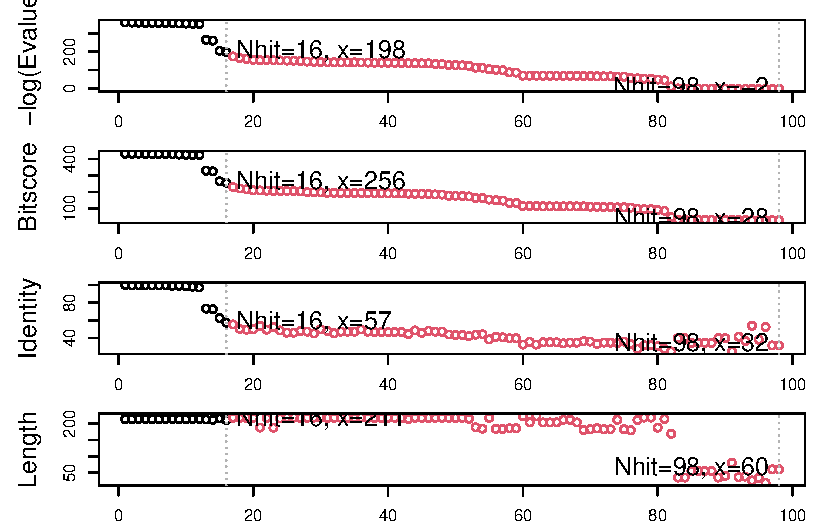
\includegraphics{Class09_html_files/figure-pdf/unnamed-chunk-9-1.pdf}

}

\end{figure}

\begin{Shaded}
\begin{Highlighting}[]
\CommentTok{\# List out some \textquotesingle{}top hits\textquotesingle{}}
\FunctionTok{head}\NormalTok{(hits}\SpecialCharTok{$}\NormalTok{pdb.id)}
\end{Highlighting}
\end{Shaded}

\begin{verbatim}
[1] "1AKE_A" "4X8M_A" "6S36_A" "6RZE_A" "4X8H_A" "3HPR_A"
\end{verbatim}

Use these ADK structures for analysis:

\begin{Shaded}
\begin{Highlighting}[]
\NormalTok{hits }\OtherTok{\textless{}{-}} \ConstantTok{NULL}
\NormalTok{hits}\SpecialCharTok{$}\NormalTok{pdb.id }\OtherTok{\textless{}{-}} \FunctionTok{c}\NormalTok{(}\StringTok{\textquotesingle{}1AKE\_A\textquotesingle{}}\NormalTok{,}\StringTok{\textquotesingle{}6S36\_A\textquotesingle{}}\NormalTok{,}\StringTok{\textquotesingle{}6RZE\_A\textquotesingle{}}\NormalTok{,}\StringTok{\textquotesingle{}3HPR\_A\textquotesingle{}}\NormalTok{,}\StringTok{\textquotesingle{}1E4V\_A\textquotesingle{}}\NormalTok{,}\StringTok{\textquotesingle{}5EJE\_A\textquotesingle{}}\NormalTok{,}\StringTok{\textquotesingle{}1E4Y\_A\textquotesingle{}}\NormalTok{,}\StringTok{\textquotesingle{}3X2S\_A\textquotesingle{}}\NormalTok{,}\StringTok{\textquotesingle{}6HAP\_A\textquotesingle{}}\NormalTok{,}\StringTok{\textquotesingle{}6HAM\_A\textquotesingle{}}\NormalTok{,}\StringTok{\textquotesingle{}4K46\_A\textquotesingle{}}\NormalTok{,}\StringTok{\textquotesingle{}3GMT\_A\textquotesingle{}}\NormalTok{,}\StringTok{\textquotesingle{}4PZL\_A\textquotesingle{}}\NormalTok{)}
\end{Highlighting}
\end{Shaded}

Download all these PDB files from the online database

\begin{Shaded}
\begin{Highlighting}[]
\CommentTok{\# Download releated PDB files}
\NormalTok{files }\OtherTok{\textless{}{-}} \FunctionTok{get.pdb}\NormalTok{(hits}\SpecialCharTok{$}\NormalTok{pdb.id, }\AttributeTok{path=}\StringTok{"pdbs"}\NormalTok{, }\AttributeTok{split=}\ConstantTok{TRUE}\NormalTok{, }\AttributeTok{gzip=}\ConstantTok{TRUE}\NormalTok{)}
\end{Highlighting}
\end{Shaded}

\begin{verbatim}
Warning in get.pdb(hits$pdb.id, path = "pdbs", split = TRUE, gzip = TRUE): pdbs/
1AKE.pdb exists. Skipping download
\end{verbatim}

\begin{verbatim}
Warning in get.pdb(hits$pdb.id, path = "pdbs", split = TRUE, gzip = TRUE): pdbs/
6S36.pdb exists. Skipping download
\end{verbatim}

\begin{verbatim}
Warning in get.pdb(hits$pdb.id, path = "pdbs", split = TRUE, gzip = TRUE): pdbs/
6RZE.pdb exists. Skipping download
\end{verbatim}

\begin{verbatim}
Warning in get.pdb(hits$pdb.id, path = "pdbs", split = TRUE, gzip = TRUE): pdbs/
3HPR.pdb exists. Skipping download
\end{verbatim}

\begin{verbatim}
Warning in get.pdb(hits$pdb.id, path = "pdbs", split = TRUE, gzip = TRUE): pdbs/
1E4V.pdb exists. Skipping download
\end{verbatim}

\begin{verbatim}
Warning in get.pdb(hits$pdb.id, path = "pdbs", split = TRUE, gzip = TRUE): pdbs/
5EJE.pdb exists. Skipping download
\end{verbatim}

\begin{verbatim}
Warning in get.pdb(hits$pdb.id, path = "pdbs", split = TRUE, gzip = TRUE): pdbs/
1E4Y.pdb exists. Skipping download
\end{verbatim}

\begin{verbatim}
Warning in get.pdb(hits$pdb.id, path = "pdbs", split = TRUE, gzip = TRUE): pdbs/
3X2S.pdb exists. Skipping download
\end{verbatim}

\begin{verbatim}
Warning in get.pdb(hits$pdb.id, path = "pdbs", split = TRUE, gzip = TRUE): pdbs/
6HAP.pdb exists. Skipping download
\end{verbatim}

\begin{verbatim}
Warning in get.pdb(hits$pdb.id, path = "pdbs", split = TRUE, gzip = TRUE): pdbs/
6HAM.pdb exists. Skipping download
\end{verbatim}

\begin{verbatim}
Warning in get.pdb(hits$pdb.id, path = "pdbs", split = TRUE, gzip = TRUE): pdbs/
4K46.pdb exists. Skipping download
\end{verbatim}

\begin{verbatim}
Warning in get.pdb(hits$pdb.id, path = "pdbs", split = TRUE, gzip = TRUE): pdbs/
3GMT.pdb exists. Skipping download
\end{verbatim}

\begin{verbatim}
Warning in get.pdb(hits$pdb.id, path = "pdbs", split = TRUE, gzip = TRUE): pdbs/
4PZL.pdb exists. Skipping download
\end{verbatim}

\begin{verbatim}

  |                                                                            
  |                                                                      |   0%
  |                                                                            
  |=====                                                                 |   8%
  |                                                                            
  |===========                                                           |  15%
  |                                                                            
  |================                                                      |  23%
  |                                                                            
  |======================                                                |  31%
  |                                                                            
  |===========================                                           |  38%
  |                                                                            
  |================================                                      |  46%
  |                                                                            
  |======================================                                |  54%
  |                                                                            
  |===========================================                           |  62%
  |                                                                            
  |================================================                      |  69%
  |                                                                            
  |======================================================                |  77%
  |                                                                            
  |===========================================================           |  85%
  |                                                                            
  |=================================================================     |  92%
  |                                                                            
  |======================================================================| 100%
\end{verbatim}

\hypertarget{align-and-superpose-structures}{%
\subsubsection{Align and superpose
structures}\label{align-and-superpose-structures}}

We will use the \texttt{pdbaln()} function to align and fit the
identified structures.

\begin{Shaded}
\begin{Highlighting}[]
\CommentTok{\# Align releated PDBs}
\NormalTok{pdbs }\OtherTok{\textless{}{-}} \FunctionTok{pdbaln}\NormalTok{(files, }\AttributeTok{fit =} \ConstantTok{TRUE}\NormalTok{, }\AttributeTok{exefile=}\StringTok{"msa"}\NormalTok{)}
\end{Highlighting}
\end{Shaded}

\begin{verbatim}
Reading PDB files:
pdbs/split_chain/1AKE_A.pdb
pdbs/split_chain/6S36_A.pdb
pdbs/split_chain/6RZE_A.pdb
pdbs/split_chain/3HPR_A.pdb
pdbs/split_chain/1E4V_A.pdb
pdbs/split_chain/5EJE_A.pdb
pdbs/split_chain/1E4Y_A.pdb
pdbs/split_chain/3X2S_A.pdb
pdbs/split_chain/6HAP_A.pdb
pdbs/split_chain/6HAM_A.pdb
pdbs/split_chain/4K46_A.pdb
pdbs/split_chain/3GMT_A.pdb
pdbs/split_chain/4PZL_A.pdb
   PDB has ALT records, taking A only, rm.alt=TRUE
.   PDB has ALT records, taking A only, rm.alt=TRUE
.   PDB has ALT records, taking A only, rm.alt=TRUE
.   PDB has ALT records, taking A only, rm.alt=TRUE
..   PDB has ALT records, taking A only, rm.alt=TRUE
....   PDB has ALT records, taking A only, rm.alt=TRUE
.   PDB has ALT records, taking A only, rm.alt=TRUE
...

Extracting sequences

pdb/seq: 1   name: pdbs/split_chain/1AKE_A.pdb 
   PDB has ALT records, taking A only, rm.alt=TRUE
pdb/seq: 2   name: pdbs/split_chain/6S36_A.pdb 
   PDB has ALT records, taking A only, rm.alt=TRUE
pdb/seq: 3   name: pdbs/split_chain/6RZE_A.pdb 
   PDB has ALT records, taking A only, rm.alt=TRUE
pdb/seq: 4   name: pdbs/split_chain/3HPR_A.pdb 
   PDB has ALT records, taking A only, rm.alt=TRUE
pdb/seq: 5   name: pdbs/split_chain/1E4V_A.pdb 
pdb/seq: 6   name: pdbs/split_chain/5EJE_A.pdb 
   PDB has ALT records, taking A only, rm.alt=TRUE
pdb/seq: 7   name: pdbs/split_chain/1E4Y_A.pdb 
pdb/seq: 8   name: pdbs/split_chain/3X2S_A.pdb 
pdb/seq: 9   name: pdbs/split_chain/6HAP_A.pdb 
pdb/seq: 10   name: pdbs/split_chain/6HAM_A.pdb 
   PDB has ALT records, taking A only, rm.alt=TRUE
pdb/seq: 11   name: pdbs/split_chain/4K46_A.pdb 
   PDB has ALT records, taking A only, rm.alt=TRUE
pdb/seq: 12   name: pdbs/split_chain/3GMT_A.pdb 
pdb/seq: 13   name: pdbs/split_chain/4PZL_A.pdb 
\end{verbatim}

\begin{Shaded}
\begin{Highlighting}[]
\NormalTok{pdbs}
\end{Highlighting}
\end{Shaded}

\begin{verbatim}
                                1        .         .         .         40 
[Truncated_Name:1]1AKE_A.pdb    ----------MRIILLGAPGAGKGTQAQFIMEKYGIPQIS
[Truncated_Name:2]6S36_A.pdb    ----------MRIILLGAPGAGKGTQAQFIMEKYGIPQIS
[Truncated_Name:3]6RZE_A.pdb    ----------MRIILLGAPGAGKGTQAQFIMEKYGIPQIS
[Truncated_Name:4]3HPR_A.pdb    ----------MRIILLGAPGAGKGTQAQFIMEKYGIPQIS
[Truncated_Name:5]1E4V_A.pdb    ----------MRIILLGAPVAGKGTQAQFIMEKYGIPQIS
[Truncated_Name:6]5EJE_A.pdb    ----------MRIILLGAPGAGKGTQAQFIMEKYGIPQIS
[Truncated_Name:7]1E4Y_A.pdb    ----------MRIILLGALVAGKGTQAQFIMEKYGIPQIS
[Truncated_Name:8]3X2S_A.pdb    ----------MRIILLGAPGAGKGTQAQFIMEKYGIPQIS
[Truncated_Name:9]6HAP_A.pdb    ----------MRIILLGAPGAGKGTQAQFIMEKYGIPQIS
[Truncated_Name:10]6HAM_A.pdb   ----------MRIILLGAPGAGKGTQAQFIMEKYGIPQIS
[Truncated_Name:11]4K46_A.pdb   ----------MRIILLGAPGAGKGTQAQFIMAKFGIPQIS
[Truncated_Name:12]3GMT_A.pdb   ----------MRLILLGAPGAGKGTQANFIKEKFGIPQIS
[Truncated_Name:13]4PZL_A.pdb   TENLYFQSNAMRIILLGAPGAGKGTQAKIIEQKYNIAHIS
                                          **^*****  *******  *  *^ *  ** 
                                1        .         .         .         40 

                               41        .         .         .         80 
[Truncated_Name:1]1AKE_A.pdb    TGDMLRAAVKSGSELGKQAKDIMDAGKLVTDELVIALVKE
[Truncated_Name:2]6S36_A.pdb    TGDMLRAAVKSGSELGKQAKDIMDAGKLVTDELVIALVKE
[Truncated_Name:3]6RZE_A.pdb    TGDMLRAAVKSGSELGKQAKDIMDAGKLVTDELVIALVKE
[Truncated_Name:4]3HPR_A.pdb    TGDMLRAAVKSGSELGKQAKDIMDAGKLVTDELVIALVKE
[Truncated_Name:5]1E4V_A.pdb    TGDMLRAAVKSGSELGKQAKDIMDAGKLVTDELVIALVKE
[Truncated_Name:6]5EJE_A.pdb    TGDMLRAAVKSGSELGKQAKDIMDACKLVTDELVIALVKE
[Truncated_Name:7]1E4Y_A.pdb    TGDMLRAAVKSGSELGKQAKDIMDAGKLVTDELVIALVKE
[Truncated_Name:8]3X2S_A.pdb    TGDMLRAAVKSGSELGKQAKDIMDCGKLVTDELVIALVKE
[Truncated_Name:9]6HAP_A.pdb    TGDMLRAAVKSGSELGKQAKDIMDAGKLVTDELVIALVRE
[Truncated_Name:10]6HAM_A.pdb   TGDMLRAAIKSGSELGKQAKDIMDAGKLVTDEIIIALVKE
[Truncated_Name:11]4K46_A.pdb   TGDMLRAAIKAGTELGKQAKSVIDAGQLVSDDIILGLVKE
[Truncated_Name:12]3GMT_A.pdb   TGDMLRAAVKAGTPLGVEAKTYMDEGKLVPDSLIIGLVKE
[Truncated_Name:13]4PZL_A.pdb   TGDMIRETIKSGSALGQELKKVLDAGELVSDEFIIKIVKD
                                ****^*  ^* *^ **   *  ^*   ** *  ^^ ^*^^ 
                               41        .         .         .         80 

                               81        .         .         .         120 
[Truncated_Name:1]1AKE_A.pdb    RIAQEDCRNGFLLDGFPRTIPQADAMKEAGINVDYVLEFD
[Truncated_Name:2]6S36_A.pdb    RIAQEDCRNGFLLDGFPRTIPQADAMKEAGINVDYVLEFD
[Truncated_Name:3]6RZE_A.pdb    RIAQEDCRNGFLLDGFPRTIPQADAMKEAGINVDYVLEFD
[Truncated_Name:4]3HPR_A.pdb    RIAQEDCRNGFLLDGFPRTIPQADAMKEAGINVDYVLEFD
[Truncated_Name:5]1E4V_A.pdb    RIAQEDCRNGFLLDGFPRTIPQADAMKEAGINVDYVLEFD
[Truncated_Name:6]5EJE_A.pdb    RIAQEDCRNGFLLDGFPRTIPQADAMKEAGINVDYVLEFD
[Truncated_Name:7]1E4Y_A.pdb    RIAQEDCRNGFLLDGFPRTIPQADAMKEAGINVDYVLEFD
[Truncated_Name:8]3X2S_A.pdb    RIAQEDSRNGFLLDGFPRTIPQADAMKEAGINVDYVLEFD
[Truncated_Name:9]6HAP_A.pdb    RICQEDSRNGFLLDGFPRTIPQADAMKEAGINVDYVLEFD
[Truncated_Name:10]6HAM_A.pdb   RICQEDSRNGFLLDGFPRTIPQADAMKEAGINVDYVLEFD
[Truncated_Name:11]4K46_A.pdb   RIAQDDCAKGFLLDGFPRTIPQADGLKEVGVVVDYVIEFD
[Truncated_Name:12]3GMT_A.pdb   RLKEADCANGYLFDGFPRTIAQADAMKEAGVAIDYVLEID
[Truncated_Name:13]4PZL_A.pdb   RISKNDCNNGFLLDGVPRTIPQAQELDKLGVNIDYIVEVD
                                *^   *   *^* ** **** **  ^   *^ ^**^^* * 
                               81        .         .         .         120 

                              121        .         .         .         160 
[Truncated_Name:1]1AKE_A.pdb    VPDELIVDRIVGRRVHAPSGRVYHVKFNPPKVEGKDDVTG
[Truncated_Name:2]6S36_A.pdb    VPDELIVDKIVGRRVHAPSGRVYHVKFNPPKVEGKDDVTG
[Truncated_Name:3]6RZE_A.pdb    VPDELIVDAIVGRRVHAPSGRVYHVKFNPPKVEGKDDVTG
[Truncated_Name:4]3HPR_A.pdb    VPDELIVDRIVGRRVHAPSGRVYHVKFNPPKVEGKDDGTG
[Truncated_Name:5]1E4V_A.pdb    VPDELIVDRIVGRRVHAPSGRVYHVKFNPPKVEGKDDVTG
[Truncated_Name:6]5EJE_A.pdb    VPDELIVDRIVGRRVHAPSGRVYHVKFNPPKVEGKDDVTG
[Truncated_Name:7]1E4Y_A.pdb    VPDELIVDRIVGRRVHAPSGRVYHVKFNPPKVEGKDDVTG
[Truncated_Name:8]3X2S_A.pdb    VPDELIVDRIVGRRVHAPSGRVYHVKFNPPKVEGKDDVTG
[Truncated_Name:9]6HAP_A.pdb    VPDELIVDRIVGRRVHAPSGRVYHVKFNPPKVEGKDDVTG
[Truncated_Name:10]6HAM_A.pdb   VPDELIVDRIVGRRVHAPSGRVYHVKFNPPKVEGKDDVTG
[Truncated_Name:11]4K46_A.pdb   VADSVIVERMAGRRAHLASGRTYHNVYNPPKVEGKDDVTG
[Truncated_Name:12]3GMT_A.pdb   VPFSEIIERMSGRRTHPASGRTYHVKFNPPKVEGKDDVTG
[Truncated_Name:13]4PZL_A.pdb   VADNLLIERITGRRIHPASGRTYHTKFNPPKVADKDDVTG
                                *    ^^^ ^ *** *  *** **  ^*****  *** ** 
                              121        .         .         .         160 

                              161        .         .         .         200 
[Truncated_Name:1]1AKE_A.pdb    EELTTRKDDQEETVRKRLVEYHQMTAPLIGYYSKEAEAGN
[Truncated_Name:2]6S36_A.pdb    EELTTRKDDQEETVRKRLVEYHQMTAPLIGYYSKEAEAGN
[Truncated_Name:3]6RZE_A.pdb    EELTTRKDDQEETVRKRLVEYHQMTAPLIGYYSKEAEAGN
[Truncated_Name:4]3HPR_A.pdb    EELTTRKDDQEETVRKRLVEYHQMTAPLIGYYSKEAEAGN
[Truncated_Name:5]1E4V_A.pdb    EELTTRKDDQEETVRKRLVEYHQMTAPLIGYYSKEAEAGN
[Truncated_Name:6]5EJE_A.pdb    EELTTRKDDQEECVRKRLVEYHQMTAPLIGYYSKEAEAGN
[Truncated_Name:7]1E4Y_A.pdb    EELTTRKDDQEETVRKRLVEYHQMTAPLIGYYSKEAEAGN
[Truncated_Name:8]3X2S_A.pdb    EELTTRKDDQEETVRKRLCEYHQMTAPLIGYYSKEAEAGN
[Truncated_Name:9]6HAP_A.pdb    EELTTRKDDQEETVRKRLVEYHQMTAPLIGYYSKEAEAGN
[Truncated_Name:10]6HAM_A.pdb   EELTTRKDDQEETVRKRLVEYHQMTAPLIGYYSKEAEAGN
[Truncated_Name:11]4K46_A.pdb   EDLVIREDDKEETVLARLGVYHNQTAPLIAYYGKEAEAGN
[Truncated_Name:12]3GMT_A.pdb   EPLVQRDDDKEETVKKRLDVYEAQTKPLITYYGDWARRGA
[Truncated_Name:13]4PZL_A.pdb   EPLITRTDDNEDTVKQRLSVYHAQTAKLIDFYRNFSSTNT
                                * *  * ** *^ *  **  *   *  ** ^*         
                              161        .         .         .         200 

                              201        .         .      227 
[Truncated_Name:1]1AKE_A.pdb    T--KYAKVDGTKPVAEVRADLEKILG-
[Truncated_Name:2]6S36_A.pdb    T--KYAKVDGTKPVAEVRADLEKILG-
[Truncated_Name:3]6RZE_A.pdb    T--KYAKVDGTKPVAEVRADLEKILG-
[Truncated_Name:4]3HPR_A.pdb    T--KYAKVDGTKPVAEVRADLEKILG-
[Truncated_Name:5]1E4V_A.pdb    T--KYAKVDGTKPVAEVRADLEKILG-
[Truncated_Name:6]5EJE_A.pdb    T--KYAKVDGTKPVAEVRADLEKILG-
[Truncated_Name:7]1E4Y_A.pdb    T--KYAKVDGTKPVAEVRADLEKILG-
[Truncated_Name:8]3X2S_A.pdb    T--KYAKVDGTKPVAEVRADLEKILG-
[Truncated_Name:9]6HAP_A.pdb    T--KYAKVDGTKPVCEVRADLEKILG-
[Truncated_Name:10]6HAM_A.pdb   T--KYAKVDGTKPVCEVRADLEKILG-
[Truncated_Name:11]4K46_A.pdb   T--QYLKFDGTKAVAEVSAELEKALA-
[Truncated_Name:12]3GMT_A.pdb   E-------NGLKAPA-----YRKISG-
[Truncated_Name:13]4PZL_A.pdb   KIPKYIKINGDQAVEKVSQDIFDQLNK
                                         *                  
                              201        .         .      227 

Call:
  pdbaln(files = files, fit = TRUE, exefile = "msa")

Class:
  pdbs, fasta

Alignment dimensions:
  13 sequence rows; 227 position columns (204 non-gap, 23 gap) 

+ attr: xyz, resno, b, chain, id, ali, resid, sse, call
\end{verbatim}

\hypertarget{jump-to-pca}{%
\section{Jump to PCA}\label{jump-to-pca}}

\begin{Shaded}
\begin{Highlighting}[]
\CommentTok{\# Perform PCA}
\NormalTok{pc.xray }\OtherTok{\textless{}{-}} \FunctionTok{pca}\NormalTok{(pdbs)}
\FunctionTok{plot}\NormalTok{(pc.xray)}
\end{Highlighting}
\end{Shaded}

\begin{figure}[H]

{\centering 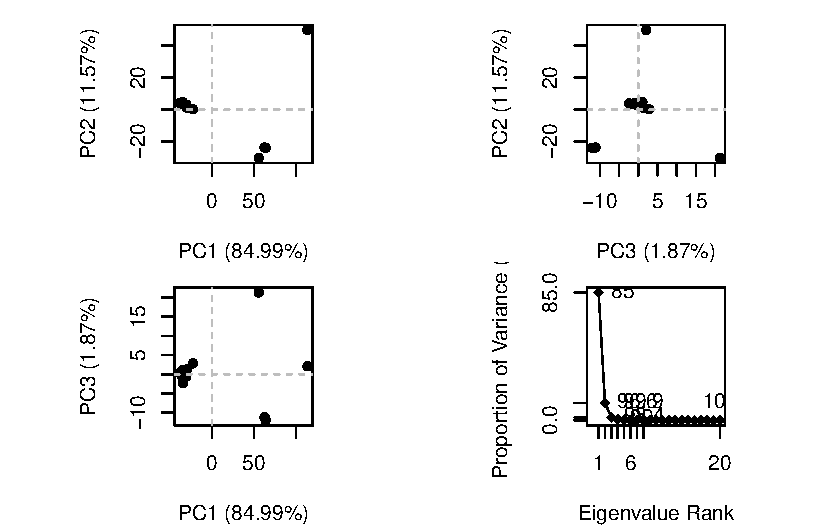
\includegraphics{Class09_html_files/figure-pdf/unnamed-chunk-14-1.pdf}

}

\end{figure}

\texttt{rmsd()} will calculate all pairwise RMSD values of the
structural ensemble. This facilitates clustering analysis based on the
pairwise structural deviation.

\begin{Shaded}
\begin{Highlighting}[]
\CommentTok{\# Calculate RMSD}
\NormalTok{rd }\OtherTok{\textless{}{-}} \FunctionTok{rmsd}\NormalTok{(pdbs)}
\end{Highlighting}
\end{Shaded}

\begin{verbatim}
Warning in rmsd(pdbs): No indices provided, using the 204 non NA positions
\end{verbatim}

\begin{Shaded}
\begin{Highlighting}[]
\CommentTok{\# Structure{-}based clustering}
\NormalTok{hc.rd }\OtherTok{\textless{}{-}} \FunctionTok{hclust}\NormalTok{(}\FunctionTok{dist}\NormalTok{(rd))}
\NormalTok{grps.rd }\OtherTok{\textless{}{-}} \FunctionTok{cutree}\NormalTok{(hc.rd, }\AttributeTok{k=}\DecValTok{3}\NormalTok{)}

\FunctionTok{plot}\NormalTok{(pc.xray, }\DecValTok{1}\SpecialCharTok{:}\DecValTok{2}\NormalTok{, }\AttributeTok{col=}\StringTok{"grey50"}\NormalTok{, }\AttributeTok{bg=}\NormalTok{grps.rd, }\AttributeTok{pch=}\DecValTok{21}\NormalTok{, }\AttributeTok{cex=}\DecValTok{1}\NormalTok{)}
\end{Highlighting}
\end{Shaded}

\begin{figure}[H]

{\centering 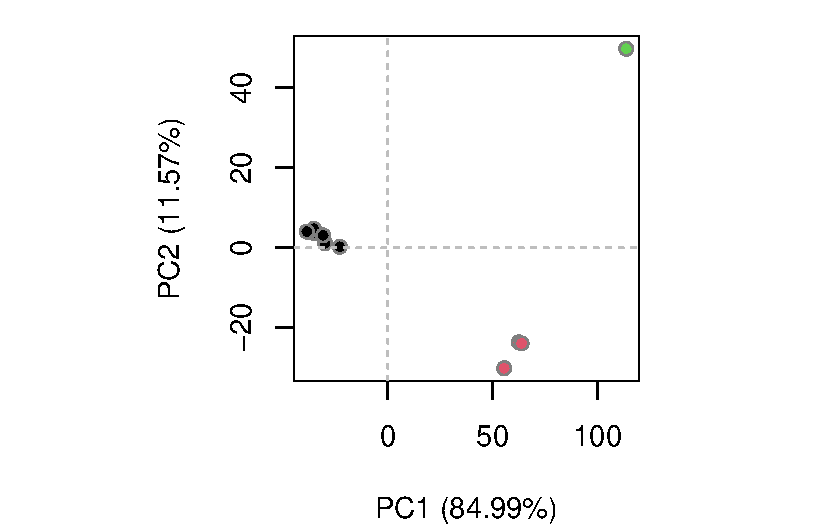
\includegraphics{Class09_html_files/figure-pdf/unnamed-chunk-15-1.pdf}

}

\end{figure}

\hypertarget{further-visualization}{%
\subsection{Further Visualization}\label{further-visualization}}

\texttt{mktrj()} can be used to generate a trajectory PDB file by
interpolating along a give PC (eigenvector):

\begin{Shaded}
\begin{Highlighting}[]
\CommentTok{\# Visualize first principal component}
\NormalTok{pc1 }\OtherTok{\textless{}{-}} \FunctionTok{mktrj}\NormalTok{(pc.xray, }\AttributeTok{pc=}\DecValTok{1}\NormalTok{, }\AttributeTok{file=}\StringTok{"pc\_1.pdb"}\NormalTok{)}
\end{Highlighting}
\end{Shaded}

\begin{itemize}
\tightlist
\item
  You can open this file, pc\_1.pdb, in Mol*.
\end{itemize}

\includegraphics{PC_1.PDB_animate-trajectory.mp4}



\end{document}
